\documentclass[letter, 10pt, journal]{elsarticle} 

\usepackage{graphicx}
\graphicspath{{figs/}}
\usepackage{paralist}

\usepackage{todonotes}  %\newcommand{\todo}[][a]{}
\usepackage{color}

%\usepackage{subfigure}
\usepackage{subcaption}
\usepackage{amssymb}
\usepackage{amsfonts}
\usepackage{bm} % for bold symbols like \bm{\alpha} or {\bm \alpha\beta}
\usepackage{mathtools}  % Fixes and additional commands for amsmath
\usepackage{cool}  % COntext-Oriented math for LaTeX
\usepackage{mleftright}  % Commands \mleft and \mright
\usepackage{booktabs}
\usepackage[per-mode=symbol]{siunitx}

% Also, note that the amsmath package sets \interdisplaylinepenalty to 10000
% thus preventing page breaks from occurring within multiline equations. Use:
\interdisplaylinepenalty=2500
% after loading amsmath to restore such page breaks

\usepackage[amsmath,thmmarks,thref]{ntheorem}
\usepackage{algpseudocode}  % Of the algorithmicx package, flexible, more math-like
\theoremstyle{definition}
\newtheorem{observation}{Observation}
\usepackage{truonglatexdefs}

\newcommand{\reviewnote}[3]{#1\footnote{\textcolor{red}{#2: #3}}}

\newcommand{\TN}[1]{\reviewnote{$\spadesuit$}{TRUONG}{#1}}
\newcommand{\MB}[1]{\reviewnote{$\diamondsuit$}{MADHUR}{#1}}
\newcommand{\RM}[1]{\reviewnote{$\heartsuit$}{RAHUL}{#1}}
\newcommand\fixme[1]{$\star$ \emph{\small #1} $\star$}
\newcommand{\eat}[1]{ }

\newcommand{\tableref}[1]{Table~\ref{tab:#1}}
\newcommand{\figref}[1]{Fig.~\ref{fig:#1}}
\newcommand{\listref}[1]{Listing~\ref{list:#1}}
% Clever references -- SHOULD BE LOADED LAST
% Generic commands: \cref and \Cref
% Seems incompatible with `algorithmic' from algorithms bundle, but can be used with `algorithmicx' (e.g. `algpseudocode').
\usepackage[capitalise]{cleveref}
\newcommand{\vref}[1]{\cref{#1}}
% When using \namecref, cleveref capitalizes the first character if the option capitalise is used, which I don't want.  So use \lcnamecref instead.

%\setlength{\textheight}{10in}
%\setlength{\textwidth}{6.8in}
%\setlength{\columnsep}{0.3125in}
%\setlength{\topmargin}{-.25in}
%\setlength{\headheight}{-.4in}
%\setlength{\headsep}{0.25in}
%\setlength{\parskip}{0cm}
%\setlength{\parindent}{1pc}
%\setlength{\partopsep}{0pt}
%\setlength{\oddsidemargin}{-.2in}

%\linespread{0.96}

%\usepackage[small]{caption}
%\usepackage{times} 
%\usepackage{flushend}
\usepackage{balance}

%\overrideIEEEmargins                                      % Needed to meet printer requirements.

\begin{document}
%
% paper title
\title{Time-Series Prediction Of The Electrocardiogram (ECG) Signal}


\author{Madhur Behl\\
Dept. of Electrical and Systems Engineering\\
University of Pennsylvania\\ 	
\{mbehl\}@seas.upenn.edu}
% conference papers do not typically use \thanks and this command
% is locked out in conference mode. If really needed, such as for
% the acknowledgment of grants, issue a \IEEEoverridecommandlockouts
% after \documentclass


% make the title area
\maketitle


%\begin{IEEEkeywords}
%
%\end{IEEEkeywords}


% For peer review papers, you can put extra information on the cover
% page as needed:
% \ifCLASSOPTIONpeerreview
% \begin{center} \bfseries EDICS Category: 3-BBND \end{center}
% \fi
%
% For peerreview papers, this IEEEtran command inserts a page break and
% creates the second title. It will be ignored for other modes.
%\IEEEpeerreviewmaketitle

\section{Autoregressive Moving Average Model (ARMA)}
Many observed time series exhibit serial autocorrelation; that is, linear association between lagged observations. This suggests past observations might predict current observations. The autoregressive (AR) process models the conditional mean of a signal $y_t$ as a function of past observations, $y_{t-1},y_{t-2},\cdots,y_{t-p}$. An autoregressive (AR) process that depends on $p$ past observations is called an AR model of degree $p$, denoted by $AR(p)$. The $AR(p)$ model is written as:
\begin{equation}
y_t = c + \psi_1 y_{t-1} + \cdots + \psi_p y_{t-p} + \epsilon_t
\end{equation}
where $\epsilon_t$ is a zero mean uncorrelated white noise term (also referred to as the innovation process term).

The moving average (MA) model captures serial autocorrelation in a time series $y_t$ by expressing the conditional mean of $y_t$ as a function of past innovations, $\epsilon_{t-1},\epsilon_{t-2},\cdots,\epsilon_{t-q}$. An MA model that depends on $q$ past innovations is called an MA model of degree $q$, denoted by $MA(q)$. The $MA(q)$ model is written as:
\begin{equation}
y_t = c + \theta_1 \epsilon_{t-1} + \cdots + \theta_q \epsilon_{t-q} 
\end{equation}

For some observed time series, a very high-order AR or MA model is needed to model the underlying process well. In this case, a combined autoregressive moving average (ARMA) model can sometimes be a more parsimonious choice. The electrocardiogram is one such example of a time-series. 
An ARMA model expresses the conditional mean of $y_t$ as a function of both past observations, $y_{t−1},y_{t−2},\cdots,y_{t−p}$, and past innovations, $\epsilon_{t−1},\epsilon_{t−2},\cdots,\epsilon_{t−q}$.
The number of past observations that $y_t$ depends on, $p$, is the AR degree. 
The number of past innovations that $y_t$ depends on, $q$, is the MA degree. 
In general, these models are denoted by $ARMA(p,q)$ and written as:

\begin{equation}
y_t = c + \psi_1 y_{t-1} + \cdots + \psi_p y_{t-p} + + \epsilon_t+ \theta_1 \epsilon_{t-1} + \cdots + \theta_q \epsilon_{t-q} 
\label{eq:arma}
\end{equation}

We use \texttt{MATLAB} to implement the $ARMA(p,q)$ models based on ~\cite{wold1954analysis,hamilton1994time}.

\section{Normal Sinus Rhythm Prediction}

We use ECG data, sampled at $2.8\si{\milli\second}$, from a healthy subject and logged for one minute to train and validate the ARMA model.
$80\%$ of the data (Figure~\ref{fig:training}) is used for training and learning the coefficients of an $ARMA(4,4)$ model (Eq.~\ref{eq:arma}).
The trained model is then used for predicting the ECG signal from the remaining $20\%$ of the data-set.
 
\begin{figure}
\centering
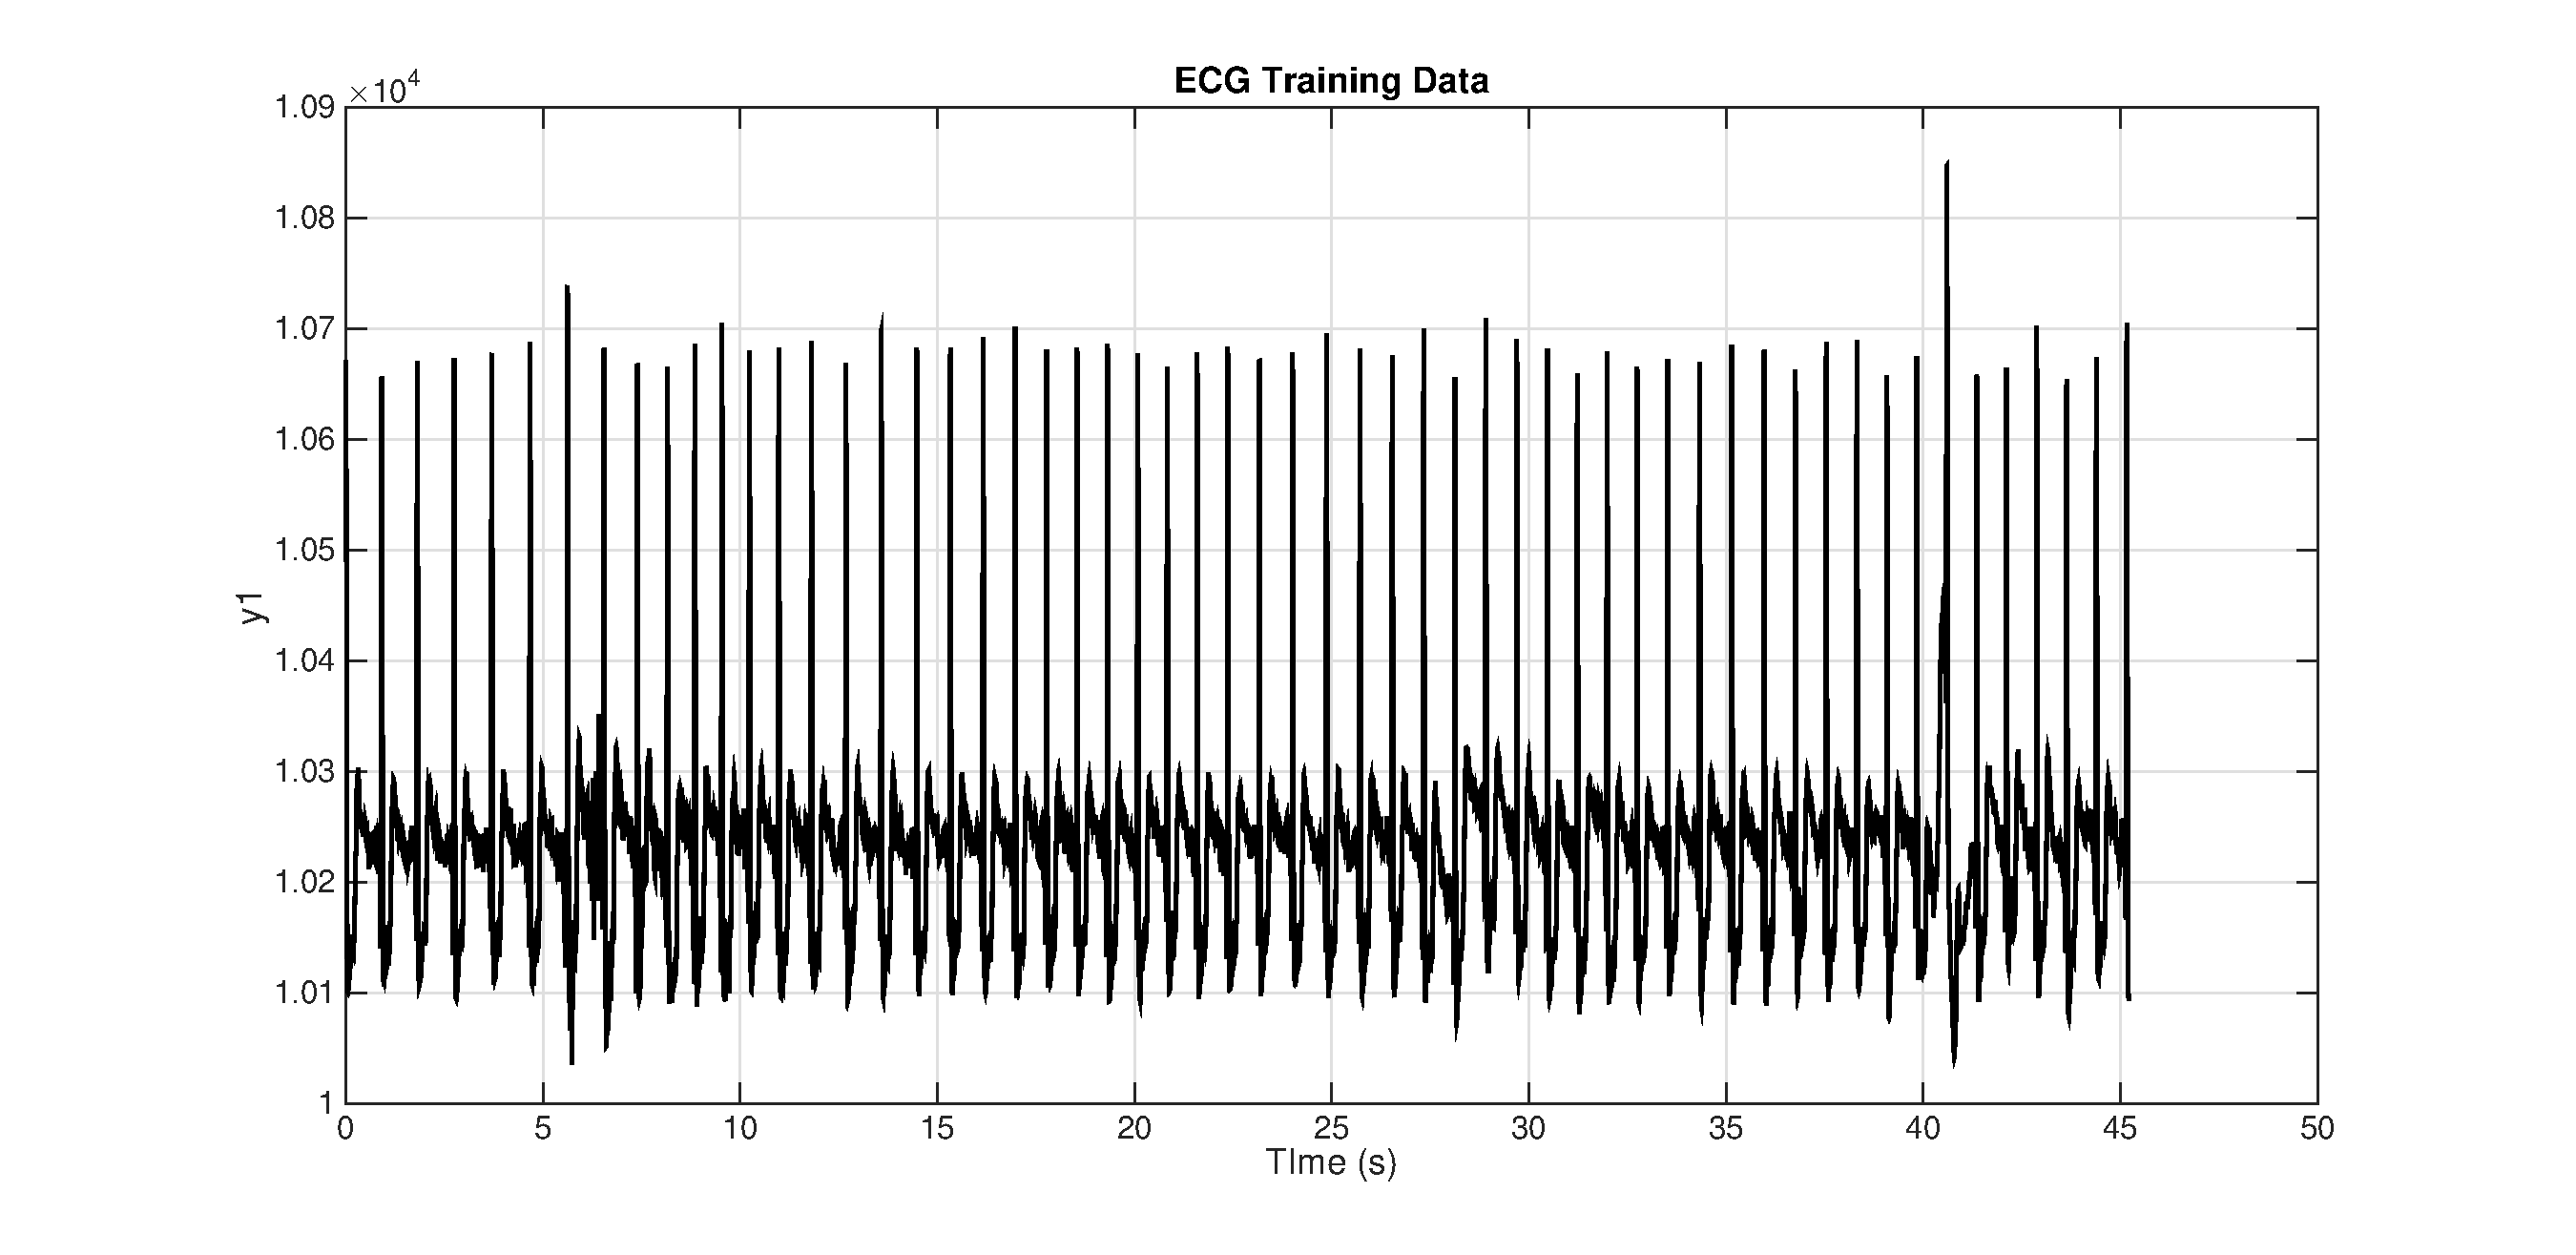
\includegraphics[width=\columnwidth]{training.eps}
\caption{Training data for the ARMA(4,4) model}
\label{fig:training}
\end{figure}

\begin{figure}[!b]
\centering
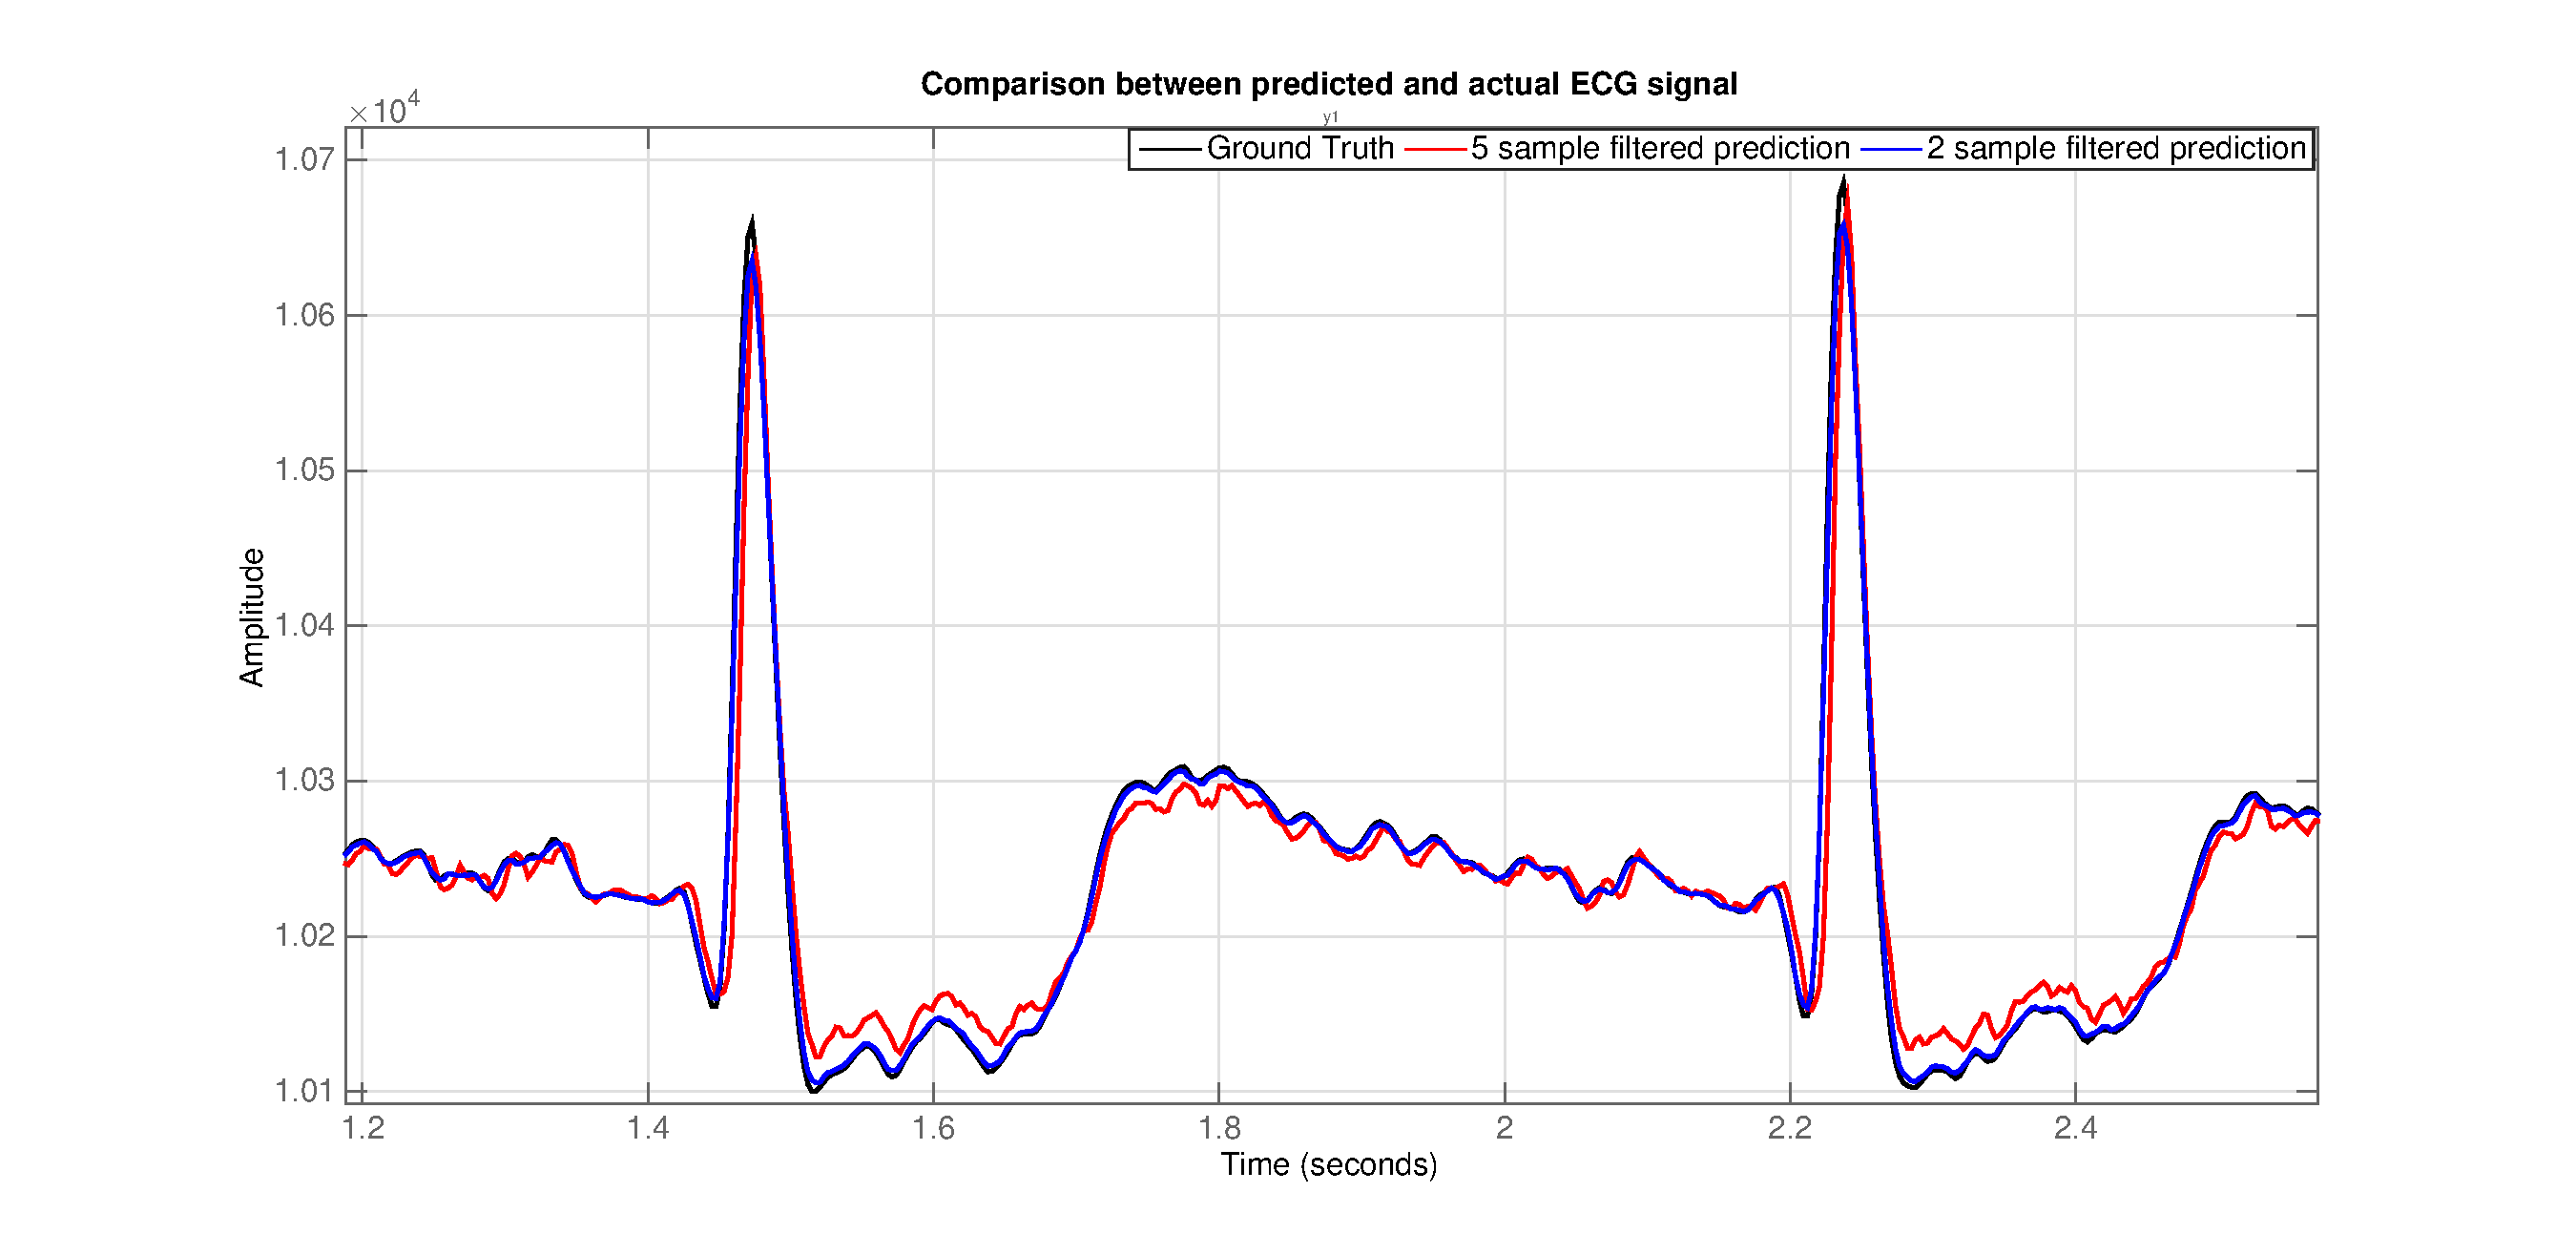
\includegraphics[width=\textwidth]{comparison.eps}
\caption{Comparison between predicted ECG response and actual ECG signal for different prediction horizons.}
\label{fig:comparison}
\end{figure}

For predicting the ECG signal, we can vary the prediction horizon. In this study, we evaluate two different prediction horizon lengths- 2 step prediction ($\sim6\si{\milli\second}$) and 5 step prediction ($\sim15\si{\milli\second}$).
The longer the prediction horizon the less accurate is the prediction.
The prediction accuracy obtained for the 2-step prediction is $92.06\%$ while a prediction accuracy of $60.36\%$ is obtained for the 5-step prediction.
The accuracy is calculated  (in percentage) as:
\begin{equation}
\text{Accuracy} = 100 \left(1 - \frac{\Vert y - \hat{y} \Vert}{\Vert y - \text{mean}(y)\Vert} \right) 
\end{equation}
The predicted response from each is further passed through a low-pass moving average filter. This helps to smooth out the predicted ECG signal and further improve the model accuracy.
Figure~\ref{fig:comparison} shows the comparison between the predicted ECG and the actual ECG signal for the filtered 2-step and 5-step prediction horizons.

\begin{figure}
\centering
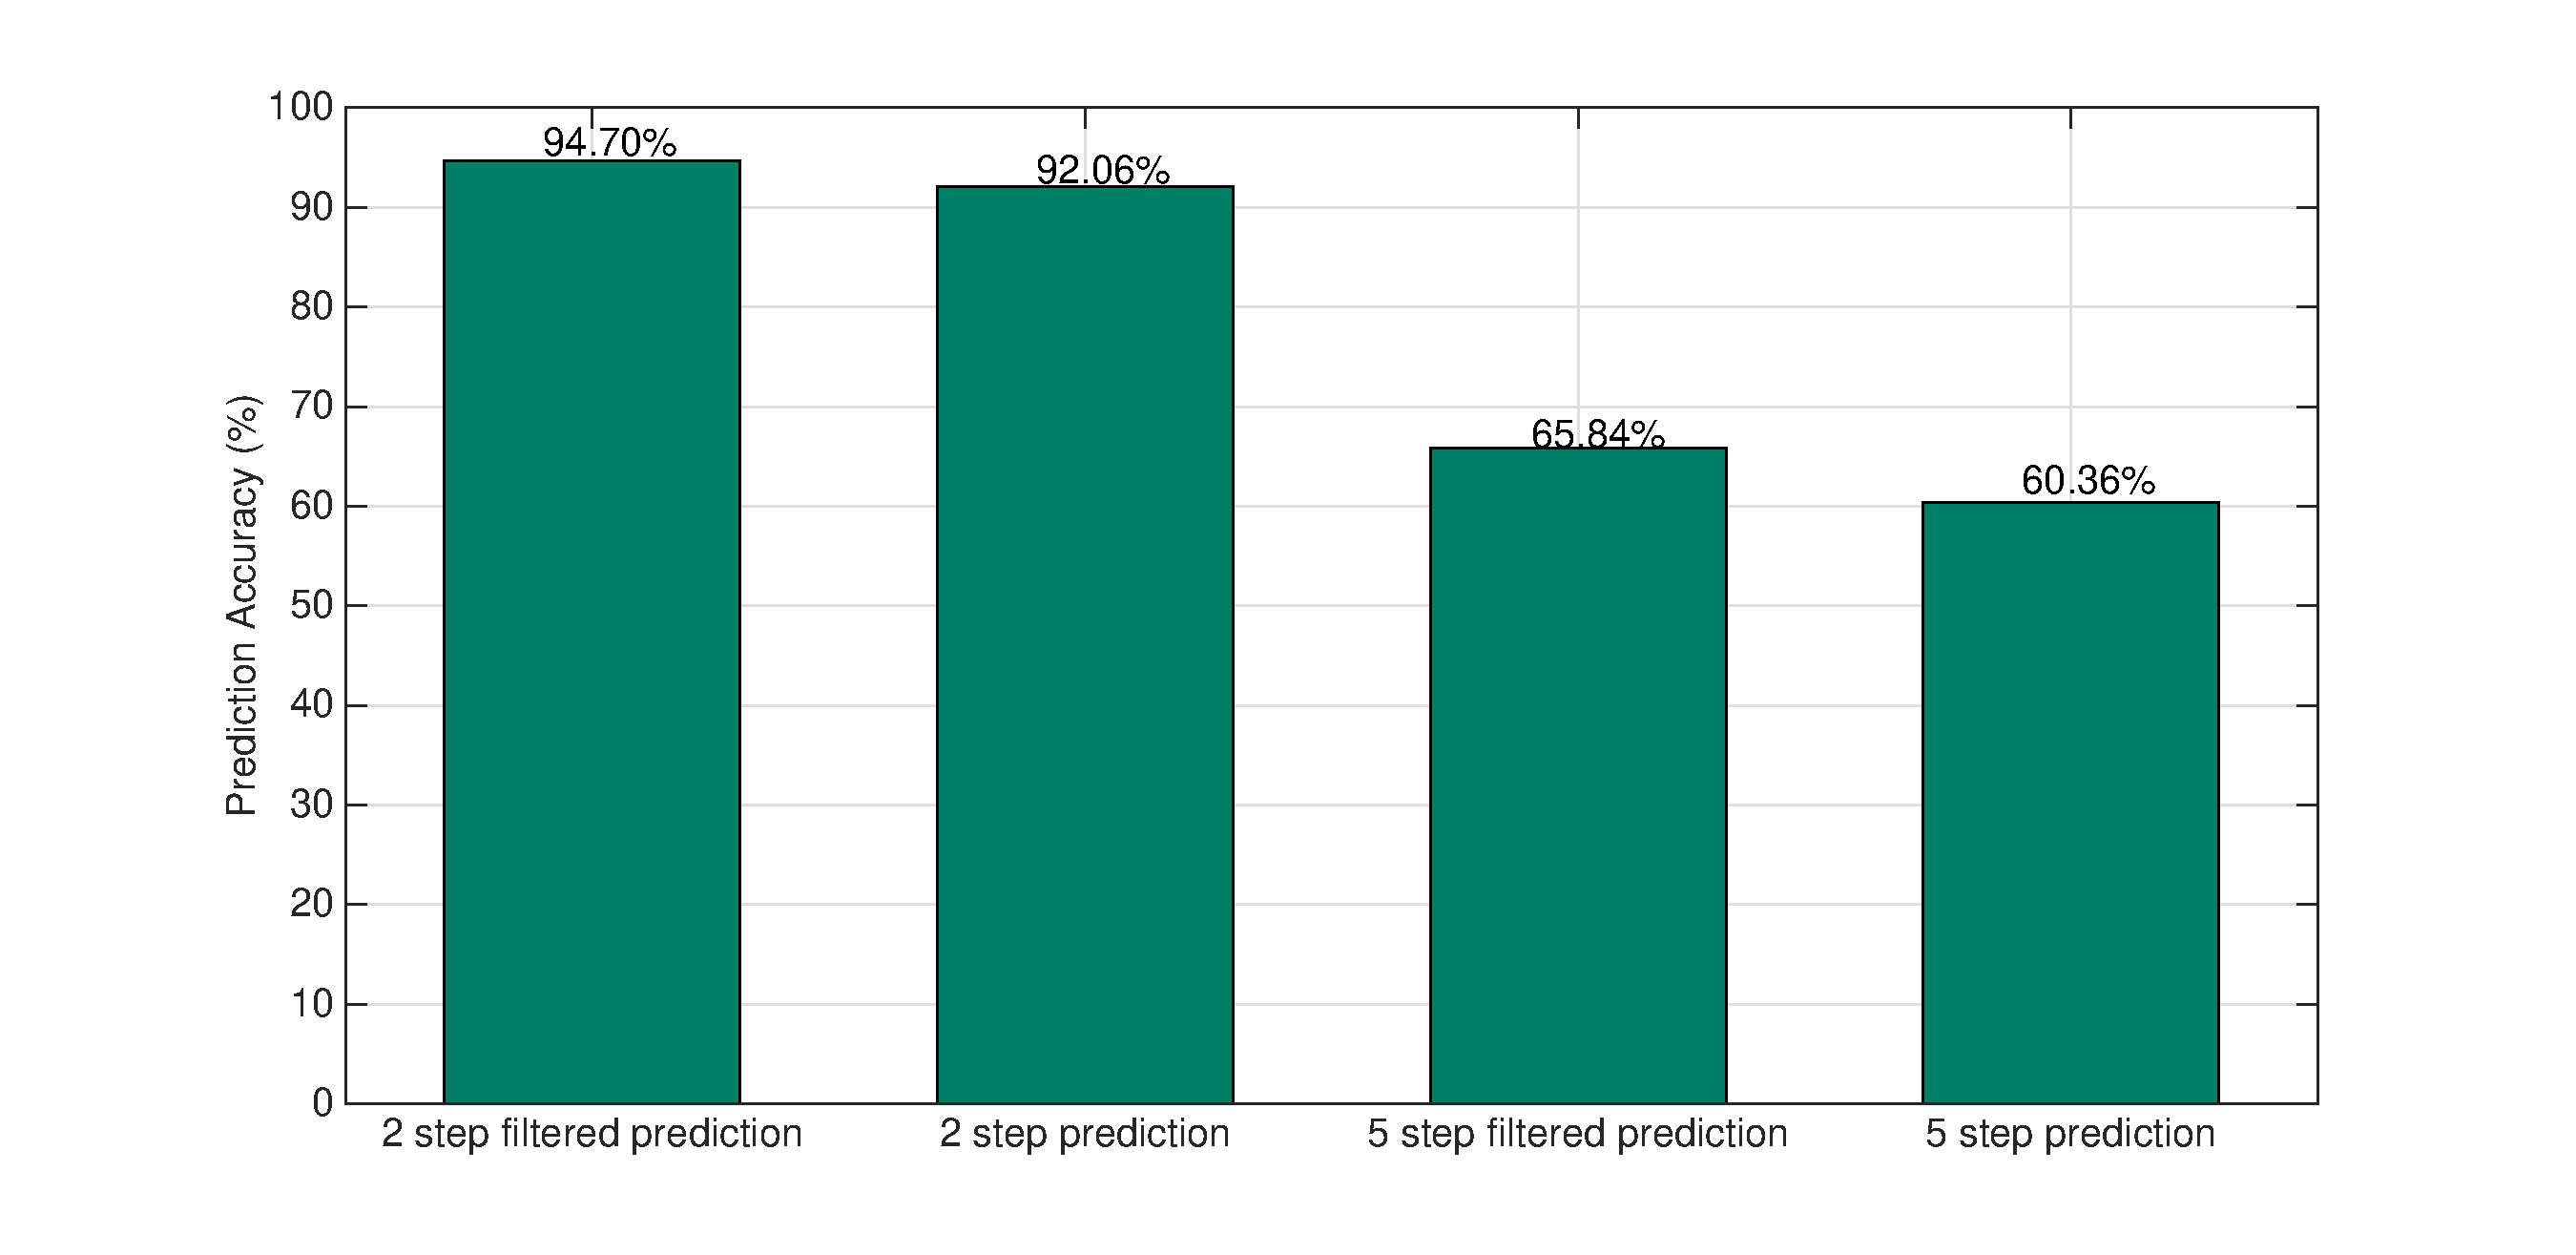
\includegraphics[width=\textwidth]{goodnessoffit.eps}
\caption{Prediction accuracy comparison for different prediction horizon lengths. Also shown is the improvement obtained by filtering the predicted response for each prediction horizon length.}
\label{fig:fit}
\end{figure}

Figure~\ref{fig:fit} shows how the prediction accuracy varies as the prediction horizon is changed from 2 to 5. We can also see that filtering the predicted response improves the prediction accuracy to $94.7\%$ from $92.06\%$ for the 2-step prediction and to $65.84\%$ from $60.36\%$ for the 5-step prediction.

Based on these preliminary results, ARMA models seem like a good choice for short term ECG prediction.
One should note that the training phase in the case-study presented in this report was completely offline. 
For a real-time implementation, the training phase can be executed after a certain number of heartbeats has been observed and stored in a buffer. The model can be continuously re-tuned and used for prediction in an online fashion.

\section{Future Work and Improvements}
So far, we have only considered NSR prediction. In the future, we will evaluate this method for prediction of ECG signals in the case of an arrhythmia present in ECG signal.
We will also investigate better methods of tuning and choosing the $p,q$ parameters of the ARMA model.
\begin{figure}
\centering
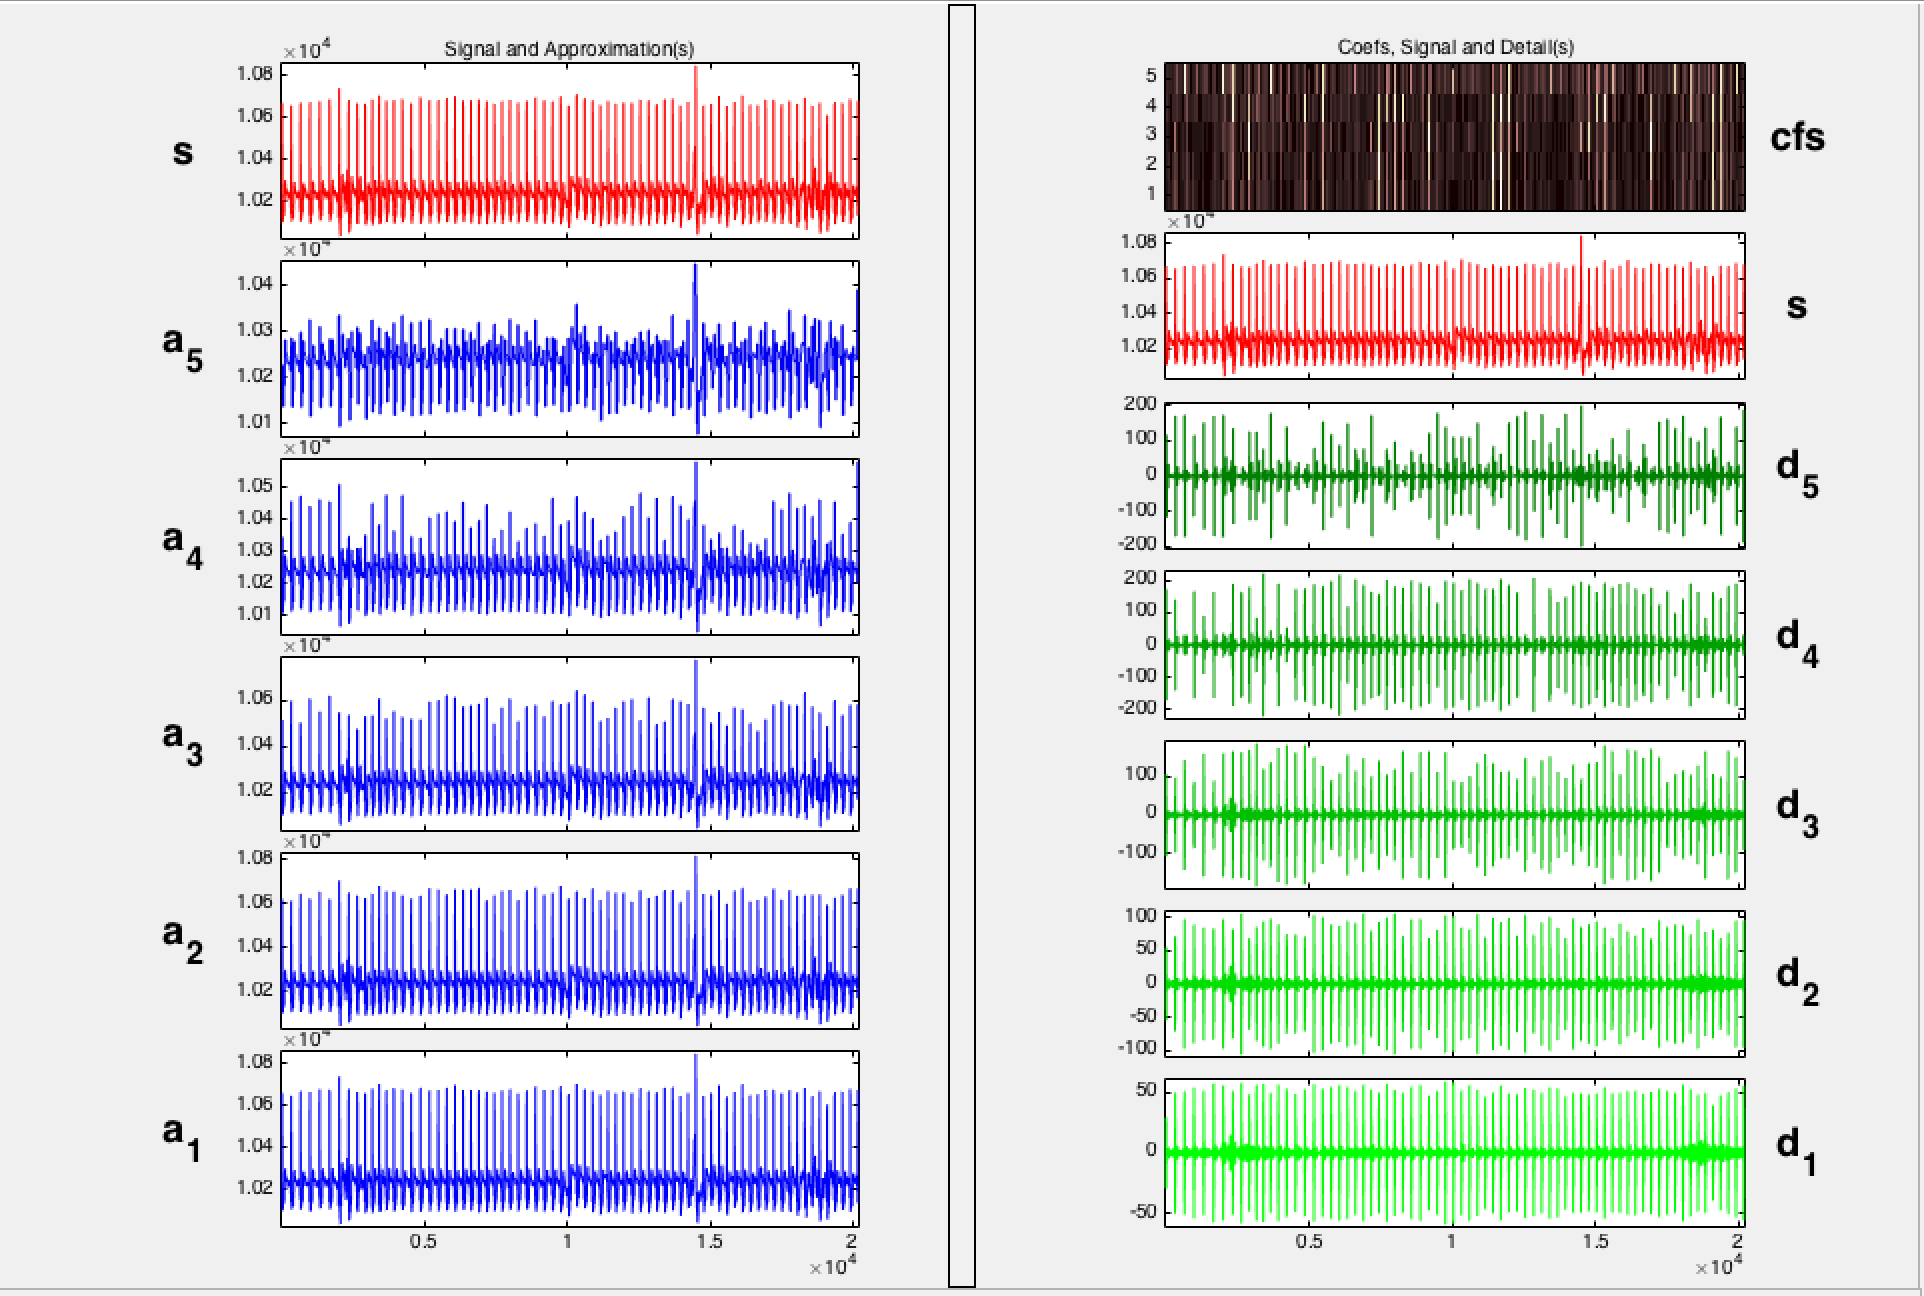
\includegraphics[width=\textwidth]{wavelet.png}
\caption{The ECG signal (s) is broken down into its approximation and detail components using Daubechies wavelets decomposition.}
\label{fig:wave}
\end{figure}

ECG signal data is non-stationary and contains transitory characteristics such as: drift, trends, abrupt changes, and beginnings and ends of events. 
These characteristics are often the most important part of the signal, and a time-series prediction is not completely suited for detecting and predicting ECG characteristics.
Using wavelet transforms, we can decompose the ECG signal into a combination of high and low frequency signals. We can then make predictions for each component and recompose the wavelets to obtain a predicted ECG signal.

Lastly, using \texttt{MATLAB}'s armax implementation it takes $2.76\si{\second}$ to train the $ARMA(4,4)$ model. This is very slow for a real-time implementation, therefore, evaluation of how fast this can be done without using \texttt{MATLAB} code will be conducted. 

\bibliographystyle{plain}
\balance
\bibliography{refs}
%
% <OR> manually copy in the resultant .bbl file
% set second argument of \begin to the number of references
% (used to reserve space for the reference number labels box)


\end{document}


